\chapter{Résultats finaux}

Après quelques essais, nous pensons avoir plutôt bien réussi notre projet. Mais il subsiste quelques défauts : une précision du capteur qui n'est pas parfaite mais satisfaisante pour une utilisation domestique, l'Arduino et son \emph{shield} ne peuvent fonctionner sans la connexion avec l'ordinateur.

Les données obtenues s'affichent très bien sur le site. Par ailleurs, nous pouvons changer la fréquence d'envoi des données.

Rappelons que vous pouvez essayez sur notre site :
\begin{itemize}
	\item le tableau à l'adresse \url{http://tpe.teguad.ovh/donnees.php} ;
	\item et le graphique à l'adresse \url{http://tpe.teguad.ovh/graphique.php}.
\end{itemize}
Il est possible de passer un argument à ces deux pages pour limiter le nombre de données (par exemple, \verb-graphique.php?limit=50- pour 50 données).

\begin{figure}[!h]
	\centering
	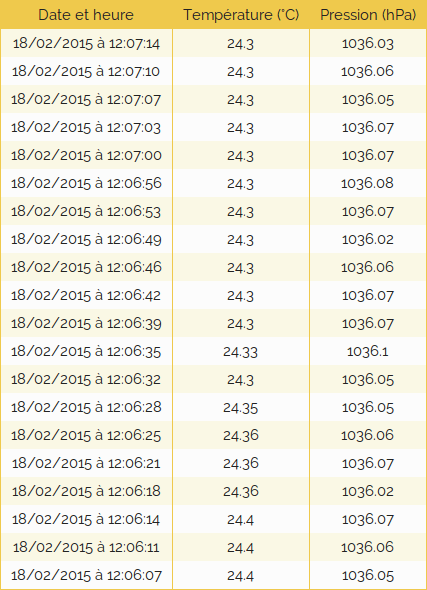
\includegraphics[scale=.5]{Images/Tableau_final}
	\caption{Aperçu du tableau finalisé}
\end{figure}

\begin{sidewaysfigure}[!h]
	\centering
	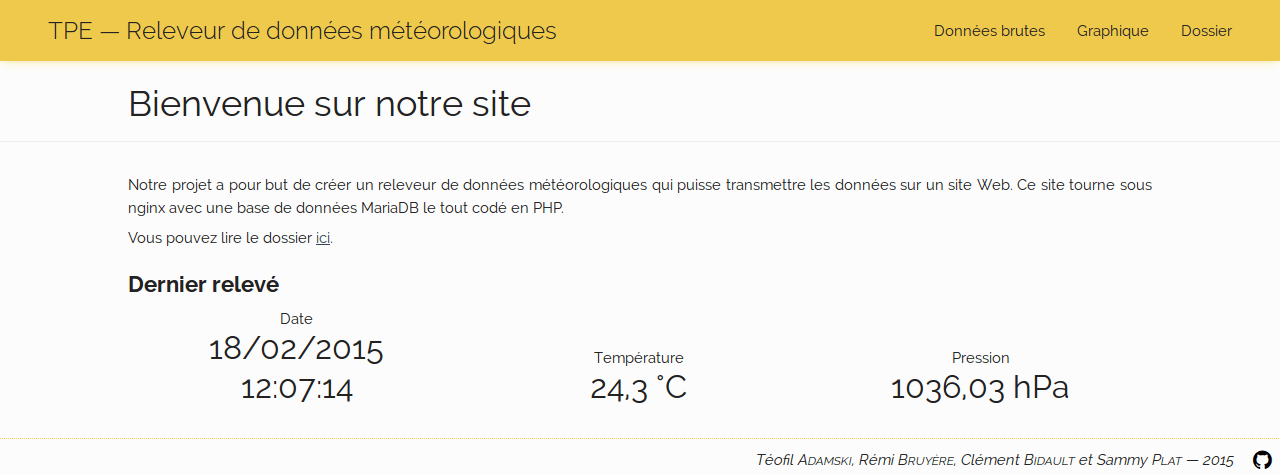
\includegraphics[width=.7\linewidth]{Images/Accueil_finale}
	\caption{Page d'accueil du site}
	\vspace{1cm}
	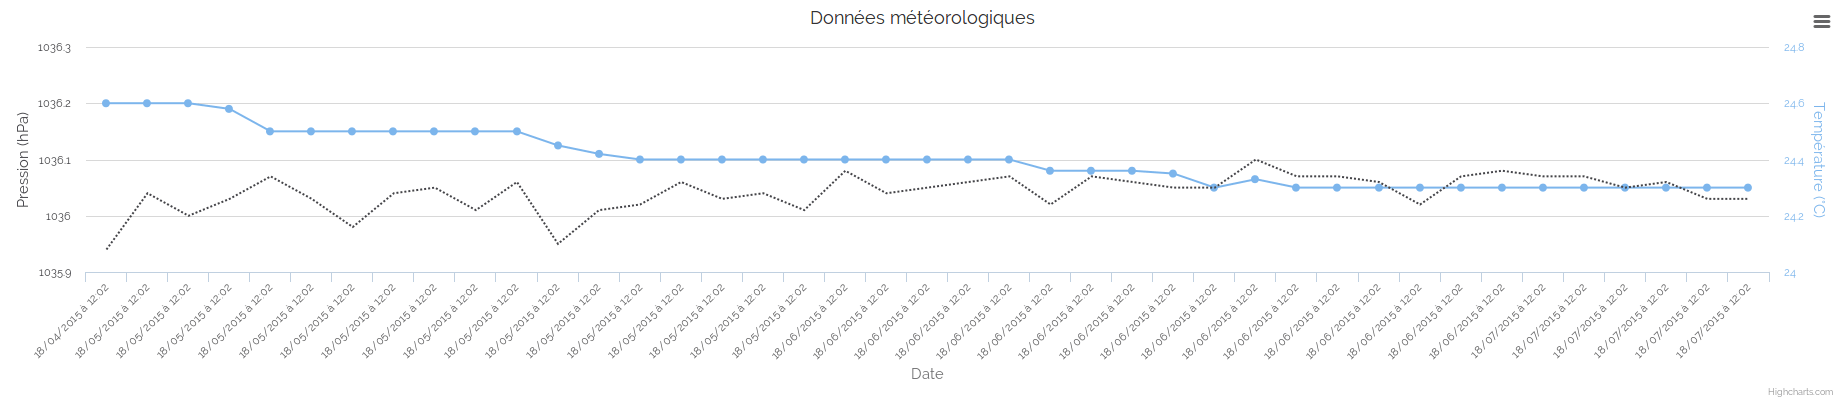
\includegraphics[width=\linewidth]{Images/Graphique_final}
	\caption{Graphique généré avec 40 relevés}
\end{sidewaysfigure}
